%%========================================================================
%% LaTeX sjabloon voor stage/projectrapport of bachelorproef
%%  HoGent Bedrijf en Organisatie
%%========================================================================

%%========================================================================
%% Preamble
%%========================================================================

\documentclass[pdftex,a4paper,12pt]{report}

% XXX: Let op: dit sjabloon is gemaakt om dubbelzijdig af te drukken
% Voor enkelzijdig, verwijder ``twoside'' hierboven.

%%---------- Extra functionaliteit ---------------------------------------

\usepackage[utf8]{inputenc}  % Accenten gebruiken in tekst (vb. é ipv \'e)
\usepackage{amsfonts}        % extra wiskundige
\usepackage{amsmath}         %   symbolen (o.a. getallen-
\usepackage{amssymb}         %   verzamelingen N, R, Z, Q, etc.)
\usepackage[dutch]{babel}    % Taalinstellingen: woordsplitsingen,
                             %  commando's voor speciale karakters
                             %  ("dutch" voor NL)
\usepackage{eurosym}         % Euro-symbool €
\usepackage{geometry}
\usepackage{graphicx}        % Invoegen van tekeningen
\usepackage{subcaption}		 % invoegen van subfiguren
\usepackage{float}			 % Positie van figuren vastleggen
\usepackage[pdftex,bookmarks=true]{hyperref}
                             % klikbare links & verwijzingen,
\usepackage{parskip}		 % Paragrafen zonder inspringen, maar witruimte
                             %  inhoudstafel
\usepackage{listings}        % Broncode mooi opmaken
\usepackage{multirow}        % Tekst over verschillende cellen in tabellen
\usepackage{rotating}        % Tabellen en figuren roteren
\usepackage{natbib}          % Betere bibliografiestijlen
\usepackage{fancyhdr}        % Pagina-opmaak met hoofd- en voettekst

\usepackage[T1]{fontenc}     % Ivm lettertypes
\usepackage{lmodern}
\usepackage{textcomp}

\usepackage{tikz}

%%---------- Layout ------------------------------------------------------
% Listing -> Code fragment
\renewcommand{\lstlistingname}{Code fragment}
\renewcommand{\lstlistlistingname}{Lijst van \lstlistingname en}% List of Listings -> List of Algorithms

% hoofdingen, enz.
\pagestyle{fancy}
% enkel hoofdstuktitel in hoofding, geen sectietitel (vermijd overlap)
\renewcommand{\sectionmark}[1]{}

% lijn, wordt gebruikt in titelpagina
\newcommand{\HRule}{\rule{\linewidth}{0.5mm}}

% Leeg blad
\newcommand{\emptypage}{
\newpage
\thispagestyle{empty}
\mbox{}
\newpage
}

% Gebruik een schreefloos lettertype ipv het "oubollig" uitziende
% Computer Modern
\renewcommand{\familydefault}{\sfdefault}

% Commando voor invoegen Java-broncodebestanden (dank aan Niels Corneille)
% Gebruik: \codefragment{source/MijnKlasse.java}{Uitleg bij de code}
\newcommand{\codefragment}[2]{ \lstset{%
  language=java,
  breaklines=true,
  float=th,
  caption={#2},
  basicstyle=\scriptsize,
  frame=single,
  extendedchars=\true
}
\lstinputlisting{#1}}

%%---------- Documenteigenschappen ---------------------------------------
%% Vul dit aan met je eigen info:

% Je eigen naam
\newcommand{\student}{Lorenz Verschingel}

% De naam van je lector, begeleider, promotor
\newcommand{\promotor}{Sabine De Vreese}

% De naam van je co-promotor
\newcommand{\copromotor}{Jean-Jacques De Clercq}

% Indien je bachelorproef in opdracht van een bedrijf of organisatie
% geschreven is, geef je hier de naam.
\newcommand{\instelling}{HoGent}

% De titel van het rapport/bachelorproef
\newcommand{\titel}{NoSQL: Cassandra}

% Datum van indienen
%TODO
\newcommand{\datum}{29 mei 2015}

% Faculteit
\newcommand{\faculteit}{Faculteit Bedrijf en Organisatie}

% Soort rapport
\newcommand{\rapporttype}{Scriptie voorgedragen tot het bekomen van de graad van\\Bachelor in de toegepaste informatica}

% Academiejaar
\newcommand{\academiejaar}{2015-2016}

% Examenperiode
%  - 1e semester = 1e examenperiode
%  - 2e semester = 2e examenperiode
%  - tweede zit = 3e examenperiode
\newcommand{\examenperiode}{Tweede examenperiode}

%%========================================================================
%% Inhoud document
%%========================================================================

\begin{document}

%%---------- Front matter ------------------------------------------------
%% Het voorblad - Hier moet je in principe niets wijzigen.

\begin{titlepage}
  \newgeometry{top=2cm,bottom=1.5cm,left=1.5cm,right=1.5cm}
  \begin{center}

    \begingroup
    \rmfamily
    
\includegraphics[width=2.5cm]{img/HG-beeldmerk-woordmerk}\\[.5cm]
    \faculteit\\[3cm]
    \titel
    \vfill
    \student\\[3.5cm]
    \rapporttype\\[2cm]
    Promotor:\\
    \promotor\\
    Co-promotor:\\
    \copromotor\\[2.5cm]
    Instelling: \instelling\\[.5cm]
    Academiejaar: \academiejaar\\[.5cm]
    \examenperiode
    \endgroup

  \end{center}
  \restoregeometry
\end{titlepage}

% Schutblad

\emptypage


\begin{titlepage}
  \newgeometry{top=5.35cm,bottom=1.5cm,left=1.5cm,right=1.5cm}
  \begin{center}

    \begingroup
    \rmfamily
    \faculteit\\[3cm]
    \titel
    \vfill
    \student\\[3.5cm]
    \rapporttype\\[2cm]
    Promotor:\\
    \promotor\\
    Co-promotor:\\
    \copromotor\\[2.5cm]
    Instelling: \instelling\\[.5cm]
    Academiejaar: \academiejaar\\[.5cm]
    \examenperiode
    \endgroup

  \end{center}
  \restoregeometry
\end{titlepage}

\begin{abstract}
% TODO: De "abstract" of samenvatting is een kernachtige (max 1 blz. voor een
% thesis) synthese van het document. In ons geval beschrijf je kort de
% probleemstelling en de context, de onderzoeksvragen, de aanpak en de
% resultaten.
In de laatste jaren zijn de NoSQL databases aan een enorme opmars bezig.
Hierbij stellen bepaalde van deze databanken hun gebruiksgemak en kunnen nogal vaak zeer positief voor.

In deze bachelorproef wordt onderzoek gedaan naar de schaalbaarheid en de betrouwbaarheid van de NoSQL database Cassandra.
Dit onderzoek wordt uitgevoerd aan de hand van een virtuele cluster die opgezet is met Vagrant.
Een ander punt dat onderzocht werd, was hoe data modellering in Cassandra in zijn werk gaat.

De schaalbaarheid wordt nagegaan door te kijken hoe gemakkelijk het is om een cluster op te zetten en om hieraan later nodes toe te voegen en weer te verwijderen.
In een virtuele omgeving is dit zeer gemakkelijk na te gaan.
Hierbij werd vastgesteld dat het opzetten van de cluster, het toevoegen van nodes en het verwijderen van nodes niet zo gemakkelijk gaat als wordt voorgesteld als men Apache Cassandra gebruikt.
Als men hier echter hulpprogramma's voor gaat gebruiken zoals het OpsCenter van DataStax gaat dit wel zeer vlot.

Om de betrouwbaarheid na te gaan werden opzettelijk nodes uitgezet om te kijken hoe Cassandra hierop reageert.
In deze testen doet Cassandra exact wat beloofd wordt.
De data blijft beschikbaar en wijzigingen worden bij het online komen van de node doorgegeven.

Bij de datamodellering werden enkele eigenaardigheden vastgesteld zoals het feit dat de primaire sleutel restricties oplegt aan de WHERE clausule.
Hierdoor moet men de data binnen Cassandra modelleren naar de query's die uitgevoerd zullen worden.

\end{abstract}

\chapter*{Voorwoord}
\label{ch:voorwoord}

% TODO: Vergeet ook niet te bedanken wie je geholpen/gesteund/... heeft
Deze bachelorproef markeert het einde van mijn driejarige opleiding Toegepaste Informatica aan de Hogeschool Gent.
Ik heb dit onderwerp, de NoSQL databank Cassandra, gekozen omdat ik er tijdens de stage mee aan de slag moest en deze technologie enorm aansprak.

Het schrijven van een bachelorproef neemt veel tijd in beslag en zonder de hulp van bepaalde mensen zou ik dit veel moeilijker tot een goed einde gebracht hebben.
Aan hen wil ik mijn grote dank uitdrukken.

Eerst en vooral wil ik de universiteit Gent bedanken voor het aanbieden van de data en in het bijzonder mijn co-promotor, de heer Jean-Jacques De Clercq, voor de technische ondersteuning en het aanhalen van het bedrijf DataStax.
Ik wil hem ook nog bedanken voor het sturen van het onderwerp in de richting van de mogelijkheden van Cassandra.

Verder wil ik ook nog mevrouw Sabine De Vreese, de promotor van deze bachelorproef bedanken voor de ondersteuning bij het opstellen van de planning en de opvolging vanuit de school.

En ten slotte wil ik ook nog mijn familie en vrienden bedanken voor de hulp bij het nalezen, de morele ondersteuning, het eenvoudig formuleren van bepaalde ingewikkelde technische aspecten\dots

Tijdens deze bachelorproef heb ik veel bijgeleerd en ik hoop dat anderen ook informatie uit deze bachelorproef zullen kunnen halen.

\vspace{4 em}

\begin{flushright}
	\textit{Lorenz Verschingel}	
\end{flushright}
\begin{flushright}
	\textit{Student Toegepaste Informatica}
\end{flushright}
\begin{flushright}
	\textit{2016}
\end{flushright}

\tableofcontents

% Als je een lijst van afkortingen of termen wil toevoegen, dan hoort die
% hier thuis. Gebruik bijvoorbeeld de ``glossaries'' package.

%%---------- Kern --------------------------------------------------------

\chapter{Inleiding}
\label{ch:inleiding}

\section{NoSQL}
Sinds de term in 1998 voor het eerst gebruikt werd door Carlo Strozzi, ging de bal aan het rollen rond NoSQL databanken.
Toen hij deze term de wereld instuurde, , doelde Strozzi met de term op een databank die op dat moment geen SQL interface aanbood.
In 2009 werd de term NoSQL opnieuw gebruikt door Johan Oskarsson als hashtag voor een meetup, waar de problemen met relationele databanken en de huidige manier van programmeren besproken gingen worden.
Nu wordt NoSQL gelezen als 'Not only SQL', wat erop wijst dat er meerdere manieren zijn om data op te slaan. \citep{Fowler2013Introduction}

NoSQL databanken vinden hun oorsprong in de moeilijkheid om objecten uit een object georiënteerd programma op te slaan in een relationele databank: de  zogenoemde 'impedance mismatch', bovendien is er het feit dat relationele databanken vaak niet goed werken op een cluster of niet met grote hoeveelheden realtime data om kunnen gaan\dots
Als gevolg hiervan maken NoSQL databanken vaak geen gebruik van een relationeel model, zijn ze gemaakt om op clusters te werken en zijn ze bovendien schema-less\dots
Kortom databanken onder de noemer NoSQL zijn aangepast om de problemen, die zich nu binnen de relationele databanken manifesteren, aan te pakken \citep{Fowler2012NoSQLDef}.

\cite{Sadalage2014OverviewNoSQL} zegt dat binnen de NoSQL databanken vier grote types naar voor geschoven kunnen worden, namelijk key-value stores (Riak, Redis\dots), document stores (MongoDB, CouchDB\dots), Column Family Stores (Cassandra, HBase\dots) en Graph databases (Neo4J, Infinite Graph\dots).
Elk van deze types heeft zijn eigen specifieke use cases.
Zelfs binnen de verschillende types NoSQL databanken komen er nog verschillende specifieke use cases voor.

%TODO CAP beter uitleggen en een figuur toevoegen
Binnen NoSQL geldt het CAP theorema.
\begin{itemize}
	\item \textbf{Consistency}: De data is op ieder moment op alle nodes gelijk
	\item \textbf{Availability}: Als een node uitvalt, dan beïnvloedt dit de andere nodes niet.
	\item \textbf{Partition Tolerance}: Het systeem blijft werken ook al zijn er netwerkfouten.
\end{itemize}

\cite{brewer2000towards} stelde dat het onmogelijk was om binnen een gedistribueerd systeem deze drie zaken samen te bekomen.
Hij gaf hiermee de aanzet dat er slechts twee van de drie punten in het CAP theorema tegelijk verkregen kunnen worden.

\section{Cassandra}

In het vervolg van deze bachelorproef wordt de focus gelegd op de NoSQL databank Cassandra.
Cassandra is een Column Family database die focust op schaalbaarheid en beschikbaarheid, zonder aan performantie in te boeten.
Cassandra is op dit moment een productiewaardige database.
Enkele bekende gebruikers van Cassandra zijn Facebook, Apple, Netflix, GitHub, Instagram, GoDaddy\dots

Cassandra is een project dat zijn oorsprong vindt bij Facebook.
In 2008 was Cassandra, bedacht door Lakshman en Malik, de oplossing voor het Inbox Search probleem van Facebook.
De moeilijkheid hierbij was dat er een systeem nodig was die eerst en vooral een hoge throughput toelaat, die daarnaast miljarden write operaties per dag moet aankunnen en die bovendien mee kan schalen met het aantal gebruikers \citep{lakshman2010cassandra}.
Om tot deze oplossing te komen baseerden Lakshman en Malik zich op twee andere projecten.

Een eerste project waarop Cassandra gebaseerd is, is Google BigTable.
Google BigTable had namelijk al een oplossing voor een eerste probleem dat Lakshman en Malik moesten oplossen: een schaalbare database die ook realtime antwoorden toelaat \citep{chang2008bigtable}.
Lakshmans vorige project, Amazon Dynamo, was de tweede inspiratiebron voor Cassandra.
Dynamo zorgde eerder al voor een hoge betrouwbaarheid bij een schaalbare database \citep{decandia2007dynamo}.

Hoewel Cassandra niet verder uitgebreid moest worden omdat het nog steeds voldeed aan de voorwaarden om het probleem van Facebook op te lossen, is Cassandra verder blijven groeien sinds 2008.
Zo kan Cassandra nu bijvoorbeeld ook overweg met gestructureerde, semi-gestructureerde en ongestructureerde data \citep{kan2014cassandra}.

Als men Cassandra binnen het CAP theorema moet gaan classificeren, kan men stellen dat de focus hier ligt op beschikbaarheid en partitie tolerantie.
Binnen Cassandra kan er toch een keuze gemaakt worden tussen snelheid en consistentie.
Hiermee kan een zeer hoge consistentie en ook een aanvaardbare snelheid verkregen worden \citep{ellis2009cassandra}.
Met het oorspronkelijk CAP theorema is dit echter niet mogelijk.
\cite{brewer2012cap} herformuleerde echter het CAP theorema omdat hij vond dat het twee-uit-drie-concept misleidend was.
Hier stelde hij dat een keuze voor de drie mogelijkheden mogelijk was als er goed nagedacht werd over de partities.

\section{Probleemstelling en onderzoeksvragen}
\label{sec:onderzoeksvragen}

% TODO: Wees zo concreet mogelijk bij het formuleren van je
% onderzoeksvra(a)g(en). Een onderzoeksvraag is trouwens iets waar nog
% niemand op dit moment een antwoord heeft (voor zover je kan nagaan).

Cassandra belooft een groot aantal zaken en binnen deze bachelorproef is het de bedoeling om deze beloften na te gaan.
Eerst en vooral zal de schaalbaarheid van Cassandra gecontroleerd worden.
Is het werkelijk eenvoudig om de database op verschillende eenvoudige servers te installeren?
Een tweede punt dat nagegaan wordt is de betrouwbaarheid van Cassandra.
Is er werkelijk geen ''single point of failure'' en in hoeverre zijn back-ups nodig binnen deze NoSQL omgeving?
Een laatste punt waarbij er stilgestaan wordt, is de data modellering in Cassandra.

\chapter{Methodologie}
\label{ch:methodologie}

% TODO: Hoe ben je te werk gegaan? Verdeel je onderzoek in grote fasen, en
% licht in elke fase toe welke stappen je gevolgd hebt. Verantwoord waarom je
% op deze manier te werk gegaan bent. Je moet kunnen aantonen dat je de best
% mogelijke manier toegepast hebt om een antwoord te vinden op de
% onderzoeksvraag.

Om een antwoord te bieden op alle onderzoeksvragen werd deze bachelorproef opgesplitst in twee luiken.
Het eerste luik omvat het eerder theoretisch gedeelte, waar een literatuurstudie aan te pas kwam.
Het tweede luik omvat het praktisch gedeelte dat nodig was om op een aantal vragen een antwoord te bieden.

In het theoretisch gedeelte komt zoals eerder vermeld de literatuurstudie aan bod.
Hierin wordt dieper ingegaan op: 
\begin{itemize} 
	\item Hoe wordt de data fysiek opgeslagen binnen Cassandra?
	\item Hoe wordt de data logisch opgeslagen binnen Cassandra?
	\item Wat wordt er juist bedoeld met het meervoudig opslaan van data?
	\item Hoe belangrijk zijn back-ups binnen dit systeem?
	\item Voor welke problemen biedt Cassandra een oplossing?
\end{itemize}

Om dit alles aan de praktijk te kunnen toetsen werd het praktisch gedeelte opgezet.
Eerst moest er een Cassandra cluster opgezet worden.
Dit gebeurde aan de hand van Vagrant virtuele machines.
Er werd geopteerd voor Vagrant omdat dit een snelle manier is om verschillende identieke virtuele machines op te zetten.
Ook kon aan de hand van één enkel script de volledige omgeving gecontroleerd worden.
Voor de installatie van Cassandra werd eerst gekozen om met de Apache versie te werken.
Het idee hiervan was om met de meest recente versie te werken.
Om praktische redenen werd later gekozen om via het OpsCenter Community Edition van DataStax te werken.
Deze tool maakte het mogelijk om via een webinterface de databank Cassandra te beheren en te observeren.
Door gebruik te maken van deze opzet konden binnen de cluster snel nodes toegevoegd of verwijderd worden en via deze opzet kon de schaalbaarheid makkelijk getest worden.

Toen deze cluster opgezet was, werd de data die aangeboden werd door de Universiteit Gent ingeladen in deze virtuele cluster.
Voor deze data kon ingeladen worden, moest er eerst stilgestaan worden bij het datamodel van deze data.
Hier werd eveneens kort stil gestaan bij het verschil tussen datamodellering binnen een relationele databank en Cassandra. 

In een laatste deel moest ook nog de betrouwbaarheid van Cassandra getest worden.
Hier werd doelbewust één van de virtuele machines (één van de nodes van de databank) uitgeschakeld om te zien hoe Cassandra hierop reageert.
Doordat dit in een virtuele omgeving gebeurde, was er geen risico op verlies van kritieke data.

%% TODO: de structuur en titel van deze hoofdstukken hangen af van je
% eigen onderzoek. Elke fase in je onderzoek kan een eigen hoofdstuk krijgen. Kies telkens een gepaste titel. ``Corpus'' is *GEEN* gepaste titel

\chapter{Opzetten van de Cassandra cluster}
\label{ch:cassandra_cluster}

\section{Apache Cassandra}
Om te beginnen aan het opzetten van de van de clusters werd geopteerd om gebruik te maken van virtuele machines, die geconfigureerd werden met Vagrant.

In een eerste poging om een werkende Cassandra cluster te bekomen werd er op elke Vagrant machine Cassandra 3.3, op moment van schrijven de meest recente versie, geïnstalleerd.
Nadat dit was gebeurd dienden nog enkele stappen te voltooid worden om een werkende cluster te bekomen \citep{DataStax2016}.
De configuratie op deze manier gaf echter veel problemen, Cassandra werd telkens na enkele bewerkingen onbruikbaar met de foutboodschap "could not access pidfile for Cassandra".
Een eerste oplossing voor dit probleem was om te zorgen dat de user cassandra toegang had tot de pidfile, want namelijk niet het geval was doordat de installatie van Cassandra werd uitgevoerd door de vagrant setup.
Maar ook dit leverde weinig resultaat op.
Wel dient opgemerkte te worden dat deze installatie van Cassandra zelf geen problemen met zich meebracht.
Voor het aanpassen van de configuratie file van Cassandra werkte deze perfect op iedere node.

\section{DataStax OpsCenter}

Uiteindelijk werd er geopteerd om gebruik te maken van OpsCenter omdat dit een gemakkelijke manier is om snel een Cassandra cluster te bekomen en omdat dit ook goede mogelijkheden tot monitoren van de database voorziet.
Van het OpsCenter werd er voor de community edition 5.2.4 gekozen.
Hiermee komt Cassandra 2.1.11 geïnstalleerd \citep{Cantoni2016}.

De setup bestaat uit 1 master node waarop het OpsCenter runt en dan 3 slave nodes waar de uiteindelijke Cassandra database op komt te runnen.
Na de NAT router van Oracle Virtual Box werd een privaat netwerk opgezet zodanig deze machines met elkaar konden communiceren.
Hiervoor moest elke machine een ip-adres krijgen binnen het netwerk en ook de /etc/hosts aangepast worden.

Eenmaal de virtuele machines correct geconfigureerd waren, werd er overgegaan tot de eigenlijke installatie van Cassandra.
Zoals eerder vermeld werd hiervoor gebruik gemaakt van het OpsCenter.
Hiervoor werd op de master node naar de localhost:8888 gesurft om de installatie te starten. Op de pagina dit te voorschijn komt werd voor de optie 'brand new cluster gekozen'.

In het volgende venster wordt er om verschillende zaken gevraagd.
Tabel \ref{tab:cas_conf} en figuur \ref{fig:cas_conf_1} geven weer hoe dit venster ingevuld werd.

\begin{table}[H]
  \begin{tabular}{|l|l|}
  \hline
  Property Name & Waarde \\
  \hline
  \hline
  Cluster Name & BP Cluster \\
  \hline
  Type & local \\
  \hline
  Package & datastax community 2.1.11 \\
  \hline
  Enpoint Snitch & GossipingPropertyFileSnitch \\
  \hline
  Username en password & vagrant/vagrant\\
  \hline
  Local Node Credentials & cassandra-node-1, cassandra-node-2, cassandra-node-3 \\
  \hline
  \end{tabular}
  \caption{Configuratie van de Cassandra Cluster}
  \label{tab:cas_conf}
\end{table}

\begin{figure}[H]
  	\centering
    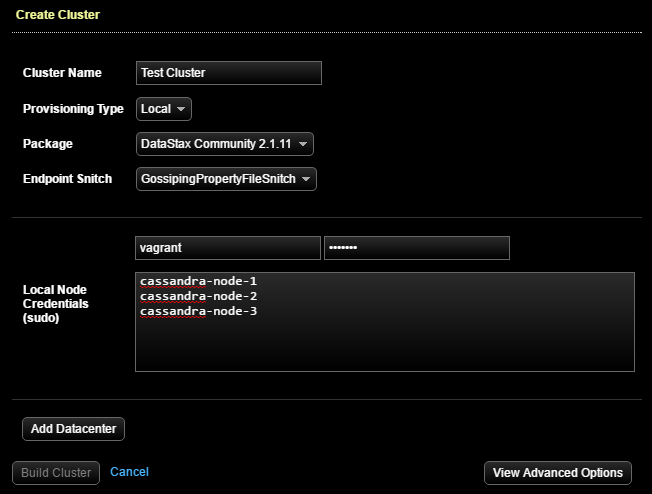
\includegraphics[width=0.5\textwidth]{img/4_installatie_cassandra/1_Configuration_part_1}
    \caption{Cassandra: Instellingen deel 1}
    \label{fig:cas_conf_1}
\end{figure}

Hier dient een datacenter toegevoegd te worden.
Hierbij wordt de naam van het datacenter vrij gekozen en zijn de node properties het ip-adres van de slave nodes (Figuur: \ref{fig:cas_conf_2}).

\begin{figure}[H]
  	\centering
    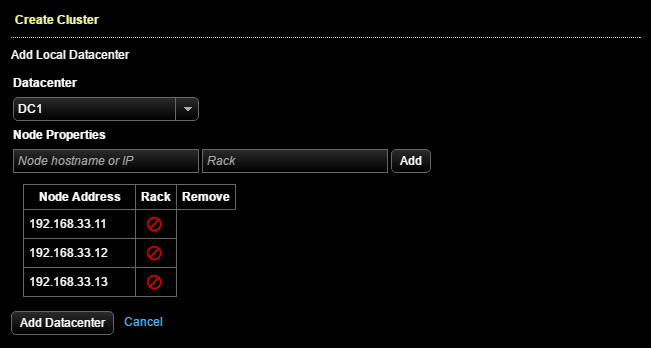
\includegraphics[width=0.5\textwidth]{img/4_installatie_cassandra/1_Configuration_part_2}
    \caption{Cassandra: Instellingen deel 2}
    \label{fig:cas_conf_2}
\end{figure}

Eenmaal de datacenters zijn toegevoegd kan men verdergaan.
Bij het drukken op de knop 'build cluster word nog gevraagd om de fingerprints van de nodes te accepteren.

Hierna begint OpsCenter met de installatie van de Cassandra cluster (Figuur: \ref{fig:cas_install}).
Deze installatie neemt enkele ogenblikken in beslag.
Als hier fouten voorkomen ligt dit veelal aan het feit dat er onvoldoende werkgeheugen aanwezig is op de slave nodes.
In de setup die hier gebruikt werd het minimum aanvaarde geheugen geven aan de slave nodes, nl 2GB.
Samen met Cassandra wordt ook de DataStax agent meegeïnstalleerd zodat het OpsCenter kan communiceren met iedere node.

\begin{figure}[H]
	\centering
	\begin{subfigure}{.49\textwidth}
  		\centering
  		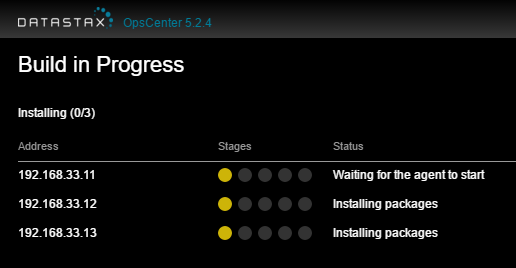
\includegraphics[width=.9\linewidth]{img/4_installatie_cassandra/1_Configuration_part_4}
  		\caption{Deel 1}
	\end{subfigure}
	\begin{subfigure}{.49\textwidth}
  		\centering
  		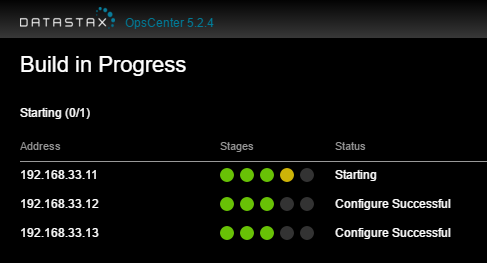
\includegraphics[width=.9\linewidth]{img/4_installatie_cassandra/1_Configuration_part_5}
  		\caption{Deel 2}
	\end{subfigure}
	\begin{subfigure}{.49\textwidth}
  		\centering
  		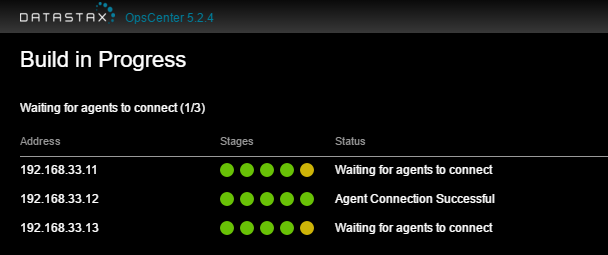
\includegraphics[width=.9\linewidth]{img/4_installatie_cassandra/1_Configuration_part_6}
  		\caption{Deel 3}
	\end{subfigure}
	\caption{Installatie van Cassandra door OpsCenter}
	\label{fig:cas_install}
\end{figure}

Na de installatie komt men terecht in het Dashboard van OpsCenter (Figuur \ref{fig:cas_opscenter_tour_dashboard}).
Hierin worden een aantal zaken weergegeven zoals de gezondheid van de cluster, het aantal write requests, de write request latency, \ldots
Hier kunnen nog meer grafieken aan toegevoegd worden via de knop "add graph".
In het tabblad nodes kan gezondheid van de cluster bekeken worden evenals hoe de data verdeeld zit over de cluster.
Deze informatie kan in ringvorm zoals op figuur \ref{fig:cas_opscenter_tour_nodes} weergegeven worden of in een lijst.

\begin{figure}[H]
	\centering
	\begin{subfigure}{.49\textwidth}
		\centering
		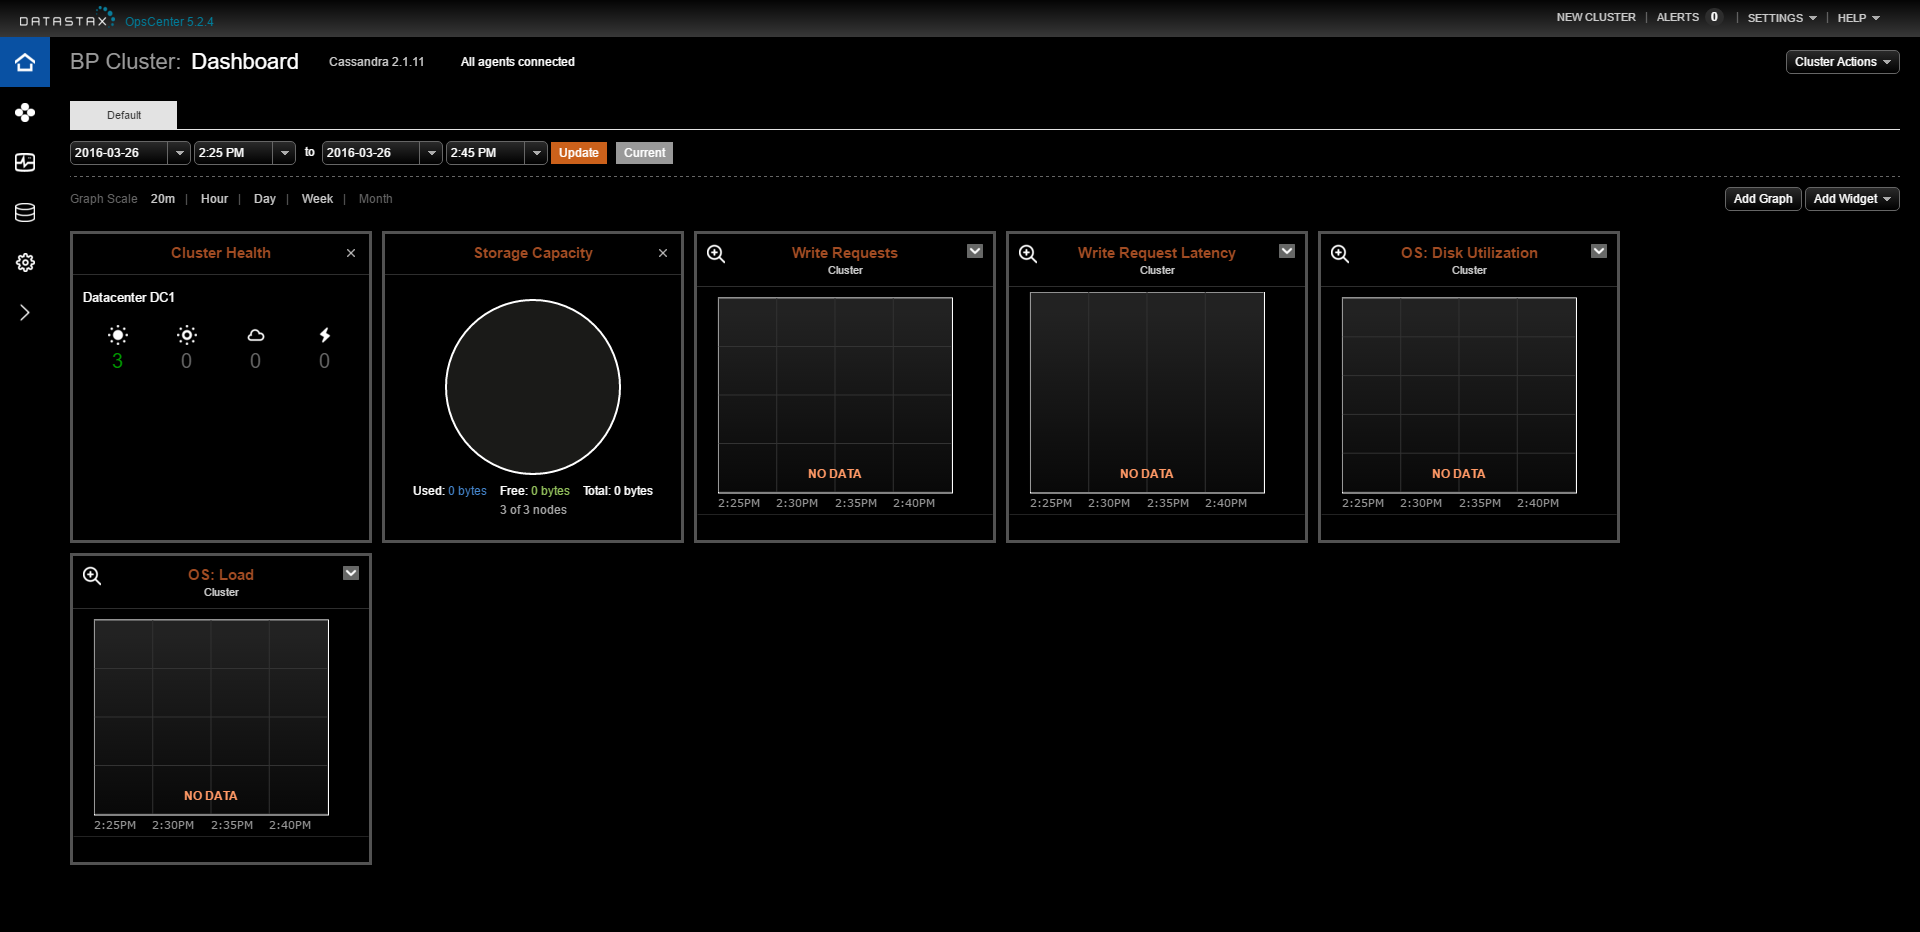
\includegraphics[width=.99\linewidth]{img/4_installatie_cassandra/2_Tour_1_Dashboard}
		\caption{Tabblad dashboard}
		\label{fig:cas_opscenter_tour_dashboard}
	\end{subfigure}
	\begin{subfigure}{.49\textwidth}
		\centering
		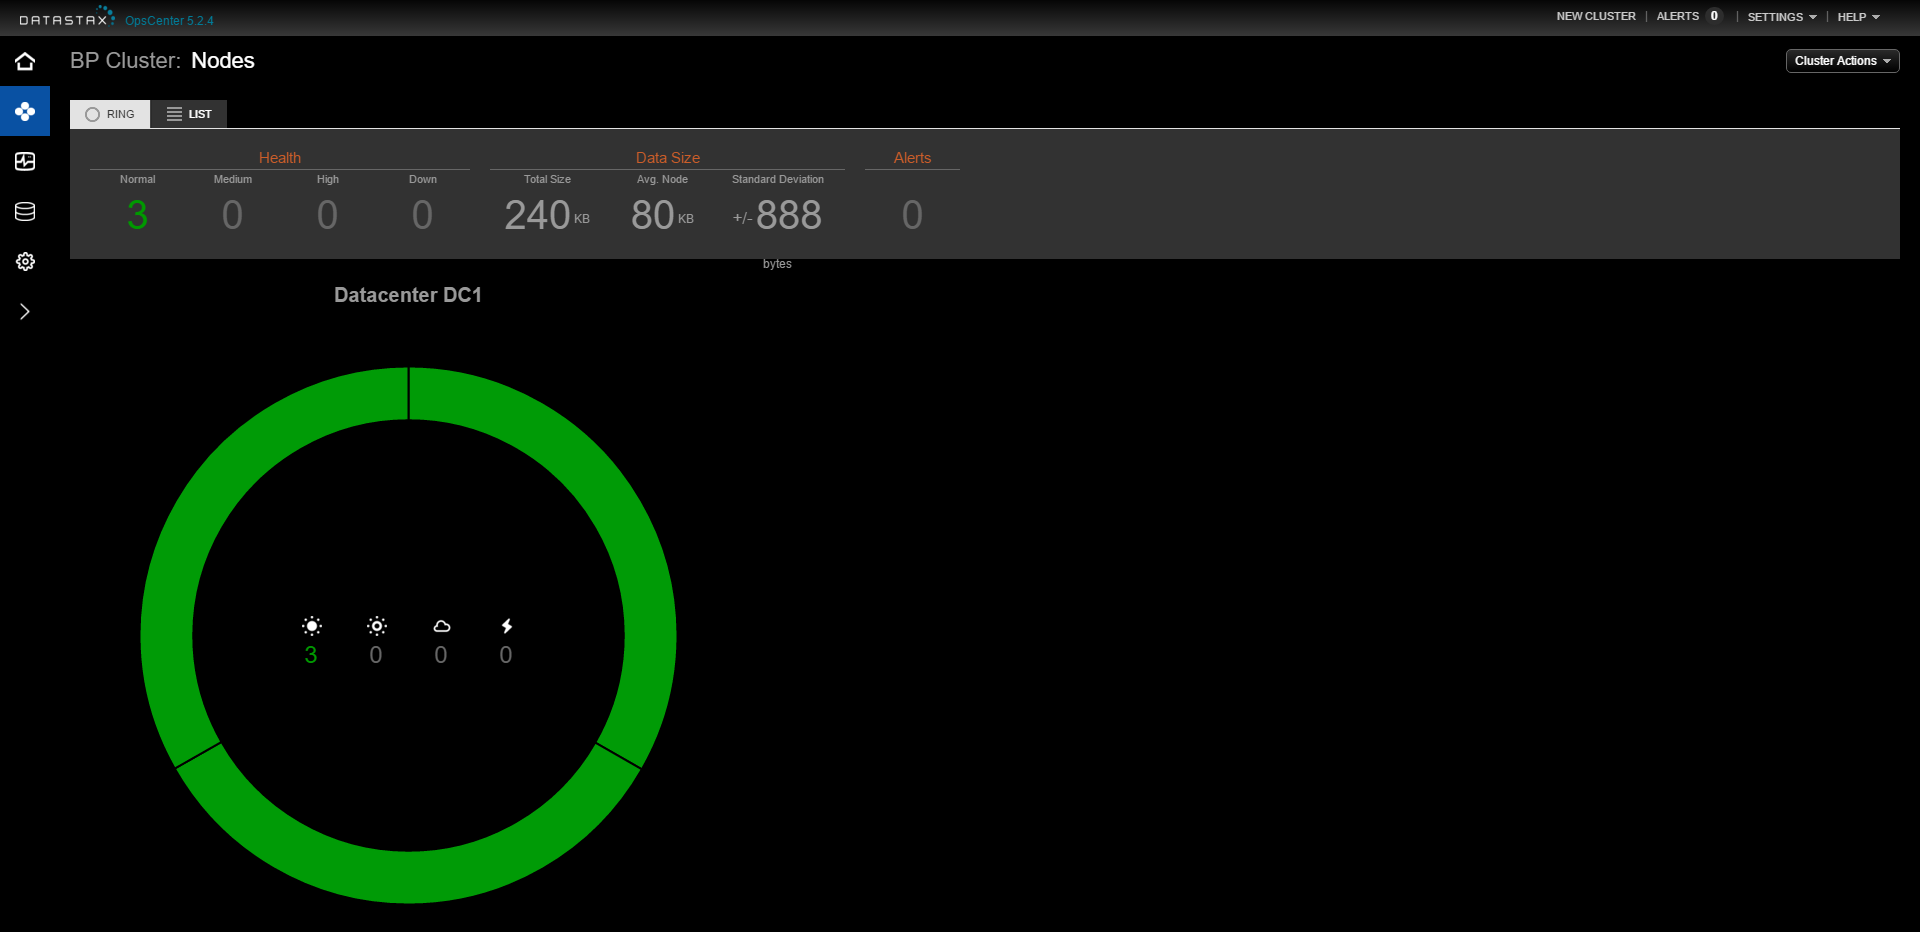
\includegraphics[width=.99\linewidth]{img/4_installatie_cassandra/2_Tour_2_Nodes}
		\caption{Tabblad nodes: ring}
		\label{fig:cas_opscenter_tour_nodes}
	\end{subfigure}
	\caption{Rondleiding in OpsCenter}
	\label{fig:cas_opscenter_tour}
\end{figure}

Cassandra voorziet zelf ook een tool die deze monitoring voorziet, nodetool.
Om te bekijken of de installatie gelukt is kan men via ssh inloggen op een van de nodes van de cluster en hier nodetool laten lopen (Figuur \ref{fig:cas_nodetool}).
Als men met nodetool de status opvraagt dan krijgt men eveneens alle nodes in de cluster te zien, samen het de hoeveelheid data die ze bevatten en hoeveel dit percentueel is van de data die aanwezig is in de cluster.

\begin{figure}[H]
	\centering
	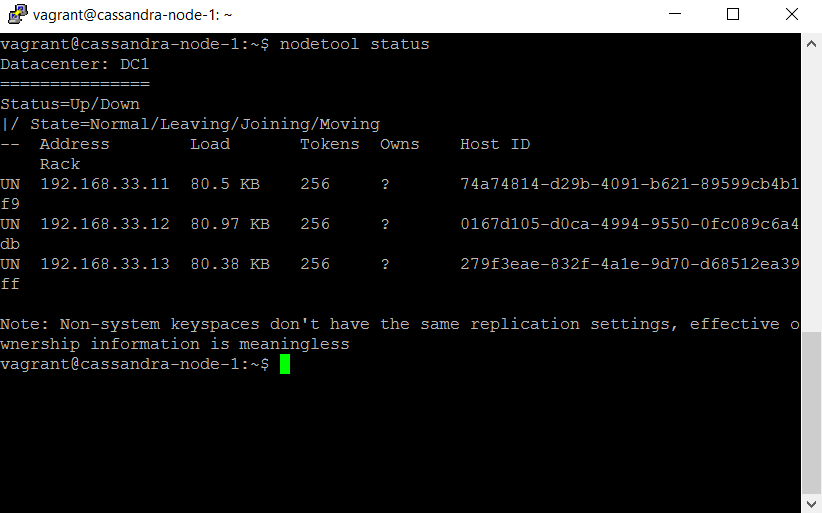
\includegraphics[width=0.5\textwidth]{img/4_installatie_cassandra/3_Node_setup}
	\caption{Nodetool}
	\label{fig:cas_nodetool}
\end{figure}

\section{Toevoegen van een node}
Het proces van het toevoegen van een node is zeer gelijkaardig aan het opzetten van de cluster.
Hierbij dient men in het OpsCenter bij het menu "cluster actions" voor de optie "add node" kiezen (Figuur \ref{fig:cas_add_node_1}).
Hier wordt een vierde node toegevoegd aan de cluster.
Net zoals bij de installatie van de cluster wordt opnieuw het scherm getoond waarin de aanmeld gegevens voor de gegeven node gevraagd worden (Figuur \ref{fig:cas_add_node_2}).
Via de knop "Add/Expand Datacenter" kan men op dezelfde manier nodes toevoegen aan het bestaande datacenter die tijdens de installatie werd aangemaakt.
Bij het bevestigen wordt opnieuw gevraagd om de fingerprint van de node te accepteren.
Hierna begint de installatie van de software op de node, de agent en cassandra worden geïnstalleerd en geconfigureerd.
Na dit alles kan men in het tabblad nodes, deze maal als een lijst, zien dat de nieuwe node is toegevoegd aan de cluster (Figuur: \ref{fig:cas_add_node_3}).

\begin{figure}[H]
	\centering
	\begin{subfigure}{.49\textwidth}
		\centering
		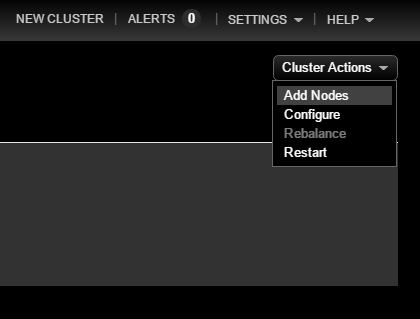
\includegraphics[width=.9\linewidth]{img/4_installatie_cassandra/4_Add_Node_1}
		\caption{Add node}
		\label{fig:cas_add_node_1}
	\end{subfigure}
	\begin{subfigure}{.49\textwidth}
		\centering
		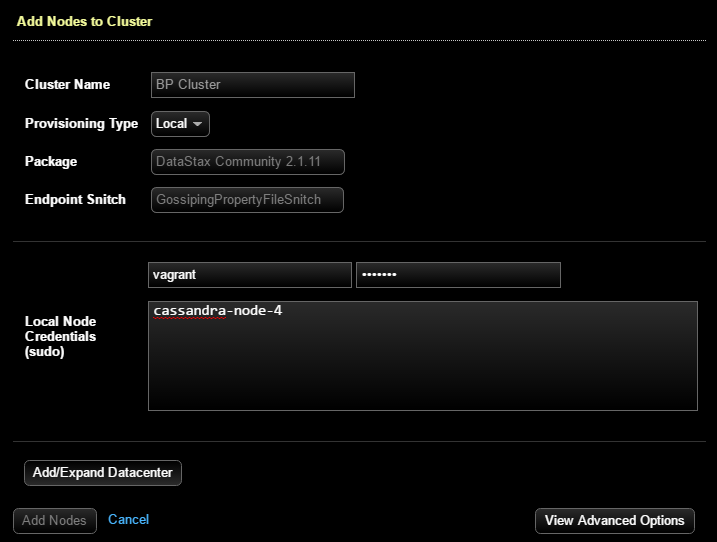
\includegraphics[width=.9\linewidth]{img/4_installatie_cassandra/4_Add_Node_2}
		\caption{Deel 2}
		\label{fig:cas_add_node_2}
	\end{subfigure}
	\begin{subfigure}{\textwidth}
		\centering
		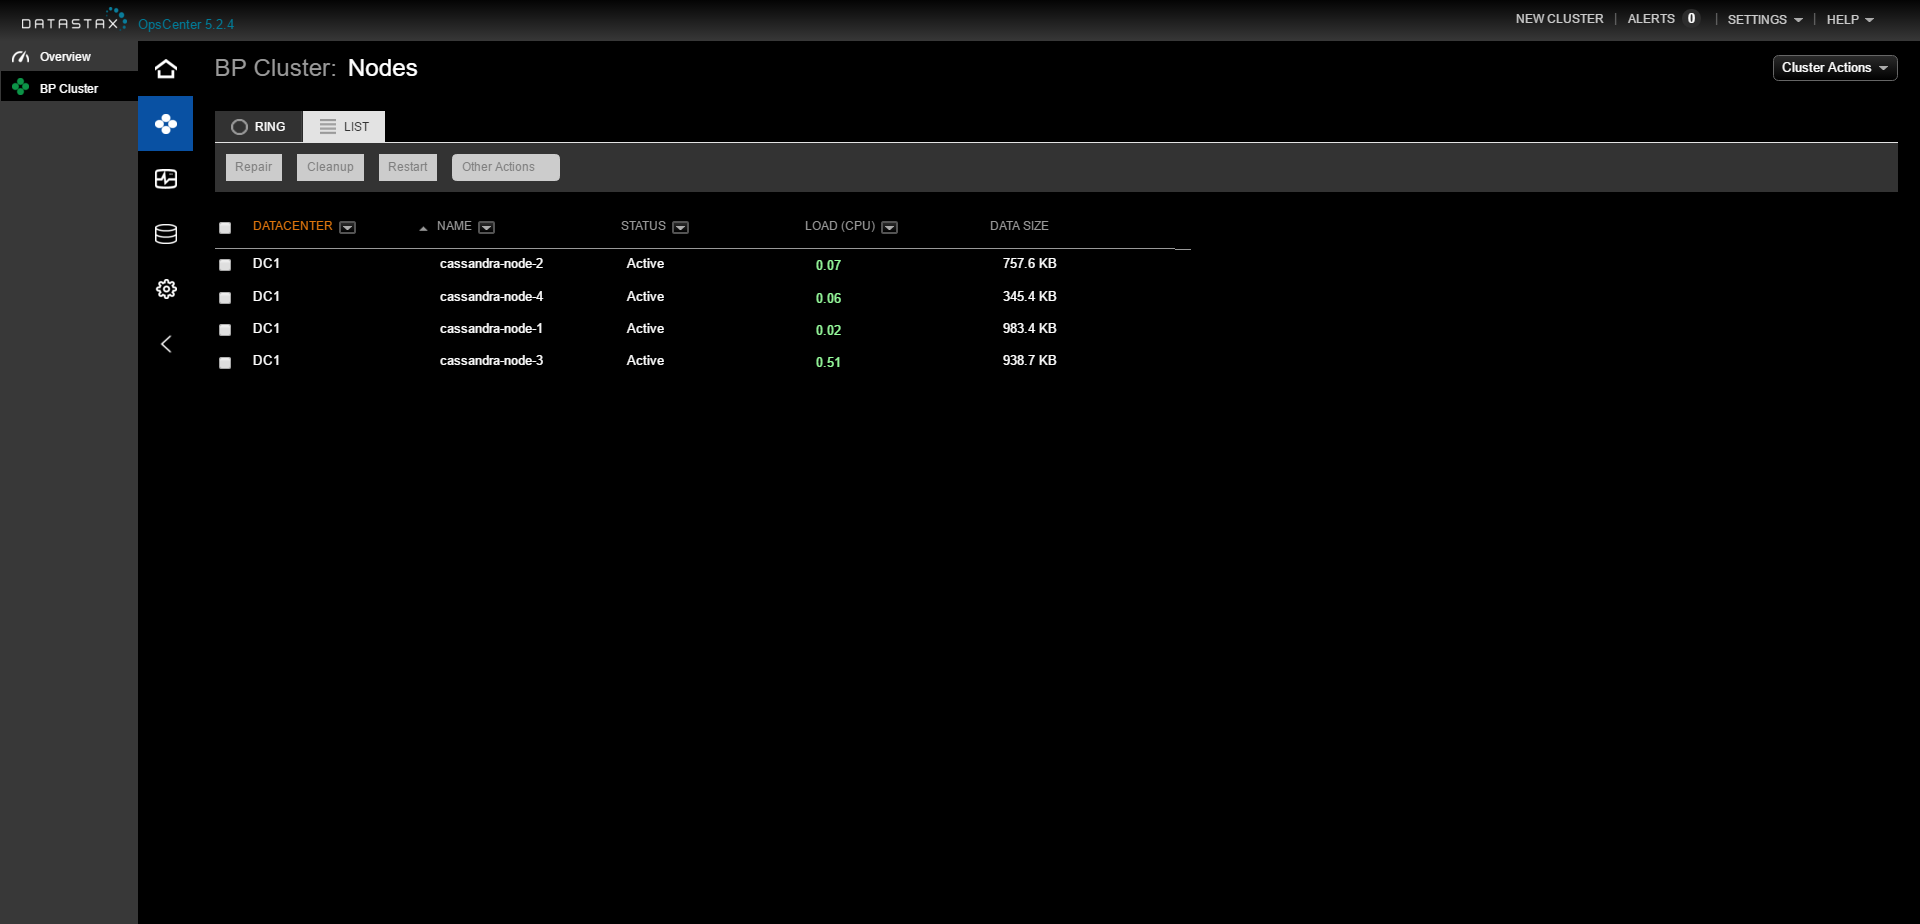
\includegraphics[width=.9\linewidth]{img/4_installatie_cassandra/4_Add_Node_7a}
		\caption{Tabblad node met 4 nodes}
		\label{fig:cas_add_node_3}
	\end{subfigure}
	\caption{Toevoegen van een node via OpsCenter}
	\label{fig:cas_add_node}
\end{figure}


\chapter{Conclusie}
\label{ch:conclusie}

% TODO: Trek een duidelijke conclusie, in de vorm van een antwoord op de
% onderzoeksvra(a)g(en). Reflecteer kritisch over het resultaat. Zijn er
% zaken die nog niet duidelijk zijn? Heeft het ondezoek geleid tot nieuwe
% vragen die uitnodigen tot verder onderzoek?

De schaalbaarheid van Cassandra werd nagegaan door nodes toe te voegen aan de cluster en het verwijderen hiervan.
Via de configuratie files van Cassandra is dit een heel karwei om te doen.
Verder werd er ook niet in geslaagd om op deze manier een werkende cluster te verkrijgen binnen deze bachelorproef.
Toen werd overgestapt naar het OpsCenter van DataStax was dit echter een ander verhaal.
Via deze weg was het zeer eenvoudig om een cluster te beheren en hier nodes aan toe te voegen of nodes te verwijderen.

Na de schaalbaarheid werd de betrouwbaarheid van de database getest.
Dit werd gedaan a.d.h.v. het uitschakelen van de nodes en zo af te toetsen of de theorie wel strookt met de werkelijkheid.
Bij uitvallen van de nodes kon telkens vastgesteld worden dat de data beschikbaar bleef.
Het hinting systeem van Cassandra bleek ook uitstekend te werken in deze test.
Toen enkel één node online was werden hier toch updates van records op uitgevoerd en bij het opnieuw opstarten van een node kon via OpsCenter vastgesteld worden dat er data uitgewisseld werd tussen de nodes.
Als men vervolgens de node, die eerst online was, uitschakelt, kan men toch de geüpdatete data terugvinden op de node die juist terug online komt.
Met het onderzoek dat in deze bachelorproef gedaan is, kan besloten worden dat Cassandra geen last heeft van ''single points of failure''.

Bij de data modellering van Cassandra zijn er toch een aantal eigenaardigheden als men vanuit een SQL omgeving komt.
Zo is het principe van modelleren naar de query's die uitgevoerd zullen worden bijzonder.
Het is echter wel nodig om hierbij stil te staan aangezien de primaire sleutel, die bestaat uit de partitie en clustering sleutel, restricties oplegt aan de WHERE clausule.
Toch is de reden waarom Cassandra deze restricties oplegt goed te begrijpen.
Want op deze manier kan de data zeer snel opgehaald worden.

Voor de back-ups kan besloten worden dat deze nog altijd nodig zijn.
De replica's zijn hier geen volwaardige vervangers voor.
Door het gebruik van replica's wordt de beschikbaarheid van de data gegarandeerd, maar dit is geen garantie tegen corrupte data.

Eén opmerking die bij dit alles moet gemaakt worden is dat alle test op virtuele machines zijn uitgevoerd en waarbij er slechts één datacenter beschikbaar was.
Door het gebruik van virtuele machines zijn de absolute tijdsgegevens in deze bachelorproef niet representatief voor een echte cluster waar de machines voor Cassandra alleen zijn voorbehouden.

Binnen het CAP theorema was de focus bij Cassandra vooral op beschikbaarheid en partitionering.
Hier slaagt Cassandra zeer goed in.
Maar meer zelf op het gebied van consistentie wordt zeer goed gescoord door de goed uitgedachte herstelmechanismes.
Met de woorden van \cite{kan2014cassandra} over wat Cassandra nu precies is kan de bachelorproef afgesloten worden, want niets in dit onderzoek kon iets van wat hij zei weerleggen.

\emph{
	''Cassandra can be simply described in a single phrase: a massively scalable, highly available open source NoSQL database that is based on peer-to-peer architecture.''
}
\citep{kan2014cassandra}


%% Citeer alle titels uit bibtex file
\nocite{*}
\bibliographystyle{apa}
\bibliography{Bachelorproef-Lorenz-Verschingel}

%%---------- Back matter -------------------------------------------------

\listoffigures
\listoftables
\lstlistoflistings

\end{document}
